\chapter{Implementation Generalized Robinson Foulds}
In this chapter we discuss the implementation for the Generalized Robinson Foulds distance. First we discuss the necessary preparation and some additional comments. These include the creation of test instances and choosing meaningful distance function. We proceed with details about the implementation and end this chapter with a short summary of the results.\\
All programs, functionalities are programmed in the programming language Python. We created a module to compute and store the Catalan numbers, create and store randomized full binary trees and finally pairwise comparing them. All implementation details can be found in my Github repository~\cite{Git}.

\section{Preparation and Overview}
The comparison of tree distances is, as already explained, a necessary tool for different research fields. But since we have to be able to find test instances that fit into the environment of the tree edit distance as well as into the one of the Robinson-Foulds distance, we are restricted to certain kinds of test data. The Robinson-Foulds distance only makes sense in the setting of phylogenetic trees on the same set of taxa, as the inner nodes aren't labelled and don't get any attention. Therefore this needs to be reflected in the tree edit distance as well. Furthermore we only take full binary trees into consideration. These are trees where every inner node has exactly two children. On the one hand this excludes multifurcations, on the other hand it ensures that any inner node represents a split between subsets of taxons.


\subsection{Creating Test Instances}
Since we hadn't found a suitable database of test instances, we needed to create it on our own. As already discussed, we have to have a set of full binary trees with pairwise differently labelled leaves. The test set needs to be a randomly selected subset of full binary trees with $n$ leaves, $n \in \mathbb{N}$.\\
Therefore we created an algorithm that chooses a full binary tree uniformly distributed which is based on the commonly known fact that the number of full binary trees with $n$ leaves is the $(n-1)$-th catalan number. Recursively, we choose the sizes of the left and the right subtrees for every inner node. In each step we need to make sure that we choose the sizes such that every possible outcome is equally possible. Before providing the algorithm, we explain the main idea with the first few recursion steps:

\begin{itemize}
\item \underline{$n=2$}: It is obvious that there is only one full binary tree with two leaves. This also fits the Catalan number $C_1=1$.
\item \underline{$n=3$}: This case is trivial as well. For the root we can decide whether the left subtree has one or two leaves. This automatically determines both subtrees. Therefore there are exactly two possible full binary trees with three leaves.
\item \underline{$n=4$}: We start with the root again. Its left subtree may contain between one and three leaves. Let's further discuss this case distinction to give an idea about the algorithm later on:
\begin{itemize}
\item \underline{Case 1}: The left subtree contains one leaf.\\
Then the left subtree needs to be a full binary tree with one leaf. The number of such trees corresponds to $C_0=1$. Furthermore the right subtree needs to contain three leaves. There are $C_2=2$ possibilities of such trees. So we end up with two different full binary trees where the left subtree of the root has only one leaf.
\item \underline{Case 2}: The left subtree contains two leaves \\
Thus the same has to hold for the right subtree. Both of them are determined since there is only $C_1=1$ such tree.
\item \underline{Case 3}: The left subtree contains three leaves.\\
 \quad This case is symmetric to the Case 1, so there are two such trees.
\end{itemize}
This results in a total number of $C_3=5$ full binary trees with four leaves. 
\end{itemize}
Our algorithm needs to make sure that choosing the number of leaves of the left and right subtrees of the root happens with correct probabilities to ensure uniform distribution among all possible full binary trees.

We exemplify the proof of uniform distribution for $n=4$ once again. Every subtree has to be chosen with probability of $\frac{1}{5} = \frac{1}{C_3}$. Trivially we have to select the Case 2, where both subtrees contain two leaves with probability $\frac{1}{5}$ since this already determines one possible outcome. The other cases are symmetric, so both of them need to be chosen with equal possibility of $\frac{2}{5}$. In both cases we have to further choose a full binary tree with three leaves. Since there are exactly two of them, we just have to make sure that both of them are chosen with probability $\frac{1}{2}$. Thus we are able to choose each full binary tree with four leaves with equal possibility.
\begin{algorithm} % enter the algorithm environment
\caption{Choosing a full binary tree with $n$ leaves with equal probability} % give the algorithm a caption
\label{alg:bin} % and a label for \ref{} commands later in the document
\begin{algorithmic}
\Function{CreateFullBinaryTree}{$n$}  
\If {$n$ == 1}
	\State \Return A single node
\Else 
	\State \textbf{var} $p$ = 0; \Comment Probability for every case
	\State \textbf{var} $P$ = 0; \Comment Sum of probabilities until now
	\State \textbf{list} $I$ = []; \Comment List of intervals between $0$ and $1$
	\For{$i = 1, (n-1)$}
		\State $p = \frac{C_{i-1} C_{n-1-i}}{C_{n-1}}$;
		\State $I[i] = [P, P+p]$;
		\State $P = P + p$;
	\EndFor
	\State $r \in [0,1)$ chosen uniformly at random;
	\State Let $j$ be the index for which $r$ lies in $I[j]$;
	\State Let $L = $ \Call{CreateFullBinaryTree}{$j$};
	\State Let $R = $ \Call{CreateFullBinaryTree}{$n-j$};
	\State \Return The binary tree with the root having the roots of $L$ and $R$ as its left and right children respectively;
\EndIf
\EndFunction
\end{algorithmic}
\end{algorithm}

\begin{lem}
Algorithm~\ref{alg:bin} returns a full binary tree with $n$ leaves, where any such tree is chosen with the same probability.
\end{lem}
\begin{proof}
We make an inductive argument:\\
\underline{Induction Base}: The routine CreateFullBinaryTree($1$) returns the only possible full binary tree with one leaf. Therefore it also gets chosen with probability 1.\\
\underline{Induction Hypothesis}: CreateFullBinaryTree($j$) returns a full binary tree with $j$ leaves chosen uniformly at random among all such trees for all $j < n$.\\
\underline{Induction Step}: $n-1 \rightarrow n$. We can assume that $n>1$, so the algorithm prepares the recursive step. First it computes some intervals. We define $p_i := \frac{C_{i-1} C_{n-1-i}}{C_{n-1}}$ as the fraction inside the for loop.\\
\textbf{Claim 1}: $P = \sum_{i=1]}^{n-1} p_i = 1$\\
\textit{Proof of Claim 1}: 
$$P = \sum_{i=1}^{n-1} p_i = \sum_{i=1}^{n-1} \frac{C_{i-1} C_{n-1-i}}{C_{n-1}} = \frac{\sum_{i=1}^{n-1} C_{i-1} C_{n-1-i}}{C_{n-1}} = \frac{\overbrace{\sum_{j=0}^{(n-1)-1} C_{j} C_{(n-1)-1-j}}^{C_{n-1}}}{C_{n-1}} = 1$$

Thus we can talk about the $p_i$'s as probabilities. The next step in the algorithm is to choose $r$ uniformly at random, which lies within the interval $I[i]$ with probability $p_i$ forall $1 \leq i < (n-1)$. The routine recursively creates the left subtree of the root with $i$ leaves and a right subtree with $n-i$ leaves. Therefore the probability is $p_i$ that we create a full binary tree, where the left subtree of the root has $i$ leaves and the right one has $n-i$ leaves. By the induction hypothesis, we know that CreateFullBinaryTree($i$) chooses a full binary tree with $i$ leaves uniformly at random. There are $C_{i-1}$ such trees, so any one of them gets chosen with probability $\frac{1}{C_{i-1}}$, analogously for $n-i$.\\
Take an arbitrarily chosen full binary tree with $n$ leaves. There exists an $1 \leq j < n$ s.t. the tree has $j$ leaves in the left subtree of the root and $n-j$ leaves in the right subtree. The probability is $p_j= \frac{C_{j-1} C_{n-1-j}}{C_{n-1}}$ that the algorithm creates a tree with these properties. Furthermore, using the induction hypothesis, it returns the left subtree with probability $\frac{1}{C_{j-1}}$ and the right one with probability $\frac{1}{C_{n-1-j}}$. All in all, the algorithm returns this arbitrary full binary tree with the following probability:
$$\underbrace{\frac{C_{j-1} C_{n-1-j}}{C_{n-1}}}_{\substack{\text{correct number of} \\ \text{leaves in}\\ \text{both subtrees}}} \quad \ \cdot \underbrace{\frac{1}{C_{j-1}}}_{\substack{\text{returning correct} \\ \text{left subtree}}} \cdot \underbrace{\frac{1}{C_{n-1-j}}}_{\substack{\text{returning correct} \\ \text{right subtree}}} = \quad \frac{1}{C_{n-1}}$$
\end{proof}
Performing this routine repeatedly allowed us to construct a uniformly randomized set of full binary trees with different numbers of leaves. We stored the test instances as Json-encoded lists of trees. We represented a tree as a recursive list with one or two elements. Take a look at the following examples:

\begin{table}[h!]
	\centering
	\begin{tabular}{c | c} 
 		Figure of tree & Python List \\
		\cmidrule(r){1-1}\cmidrule(l){2-2}
		{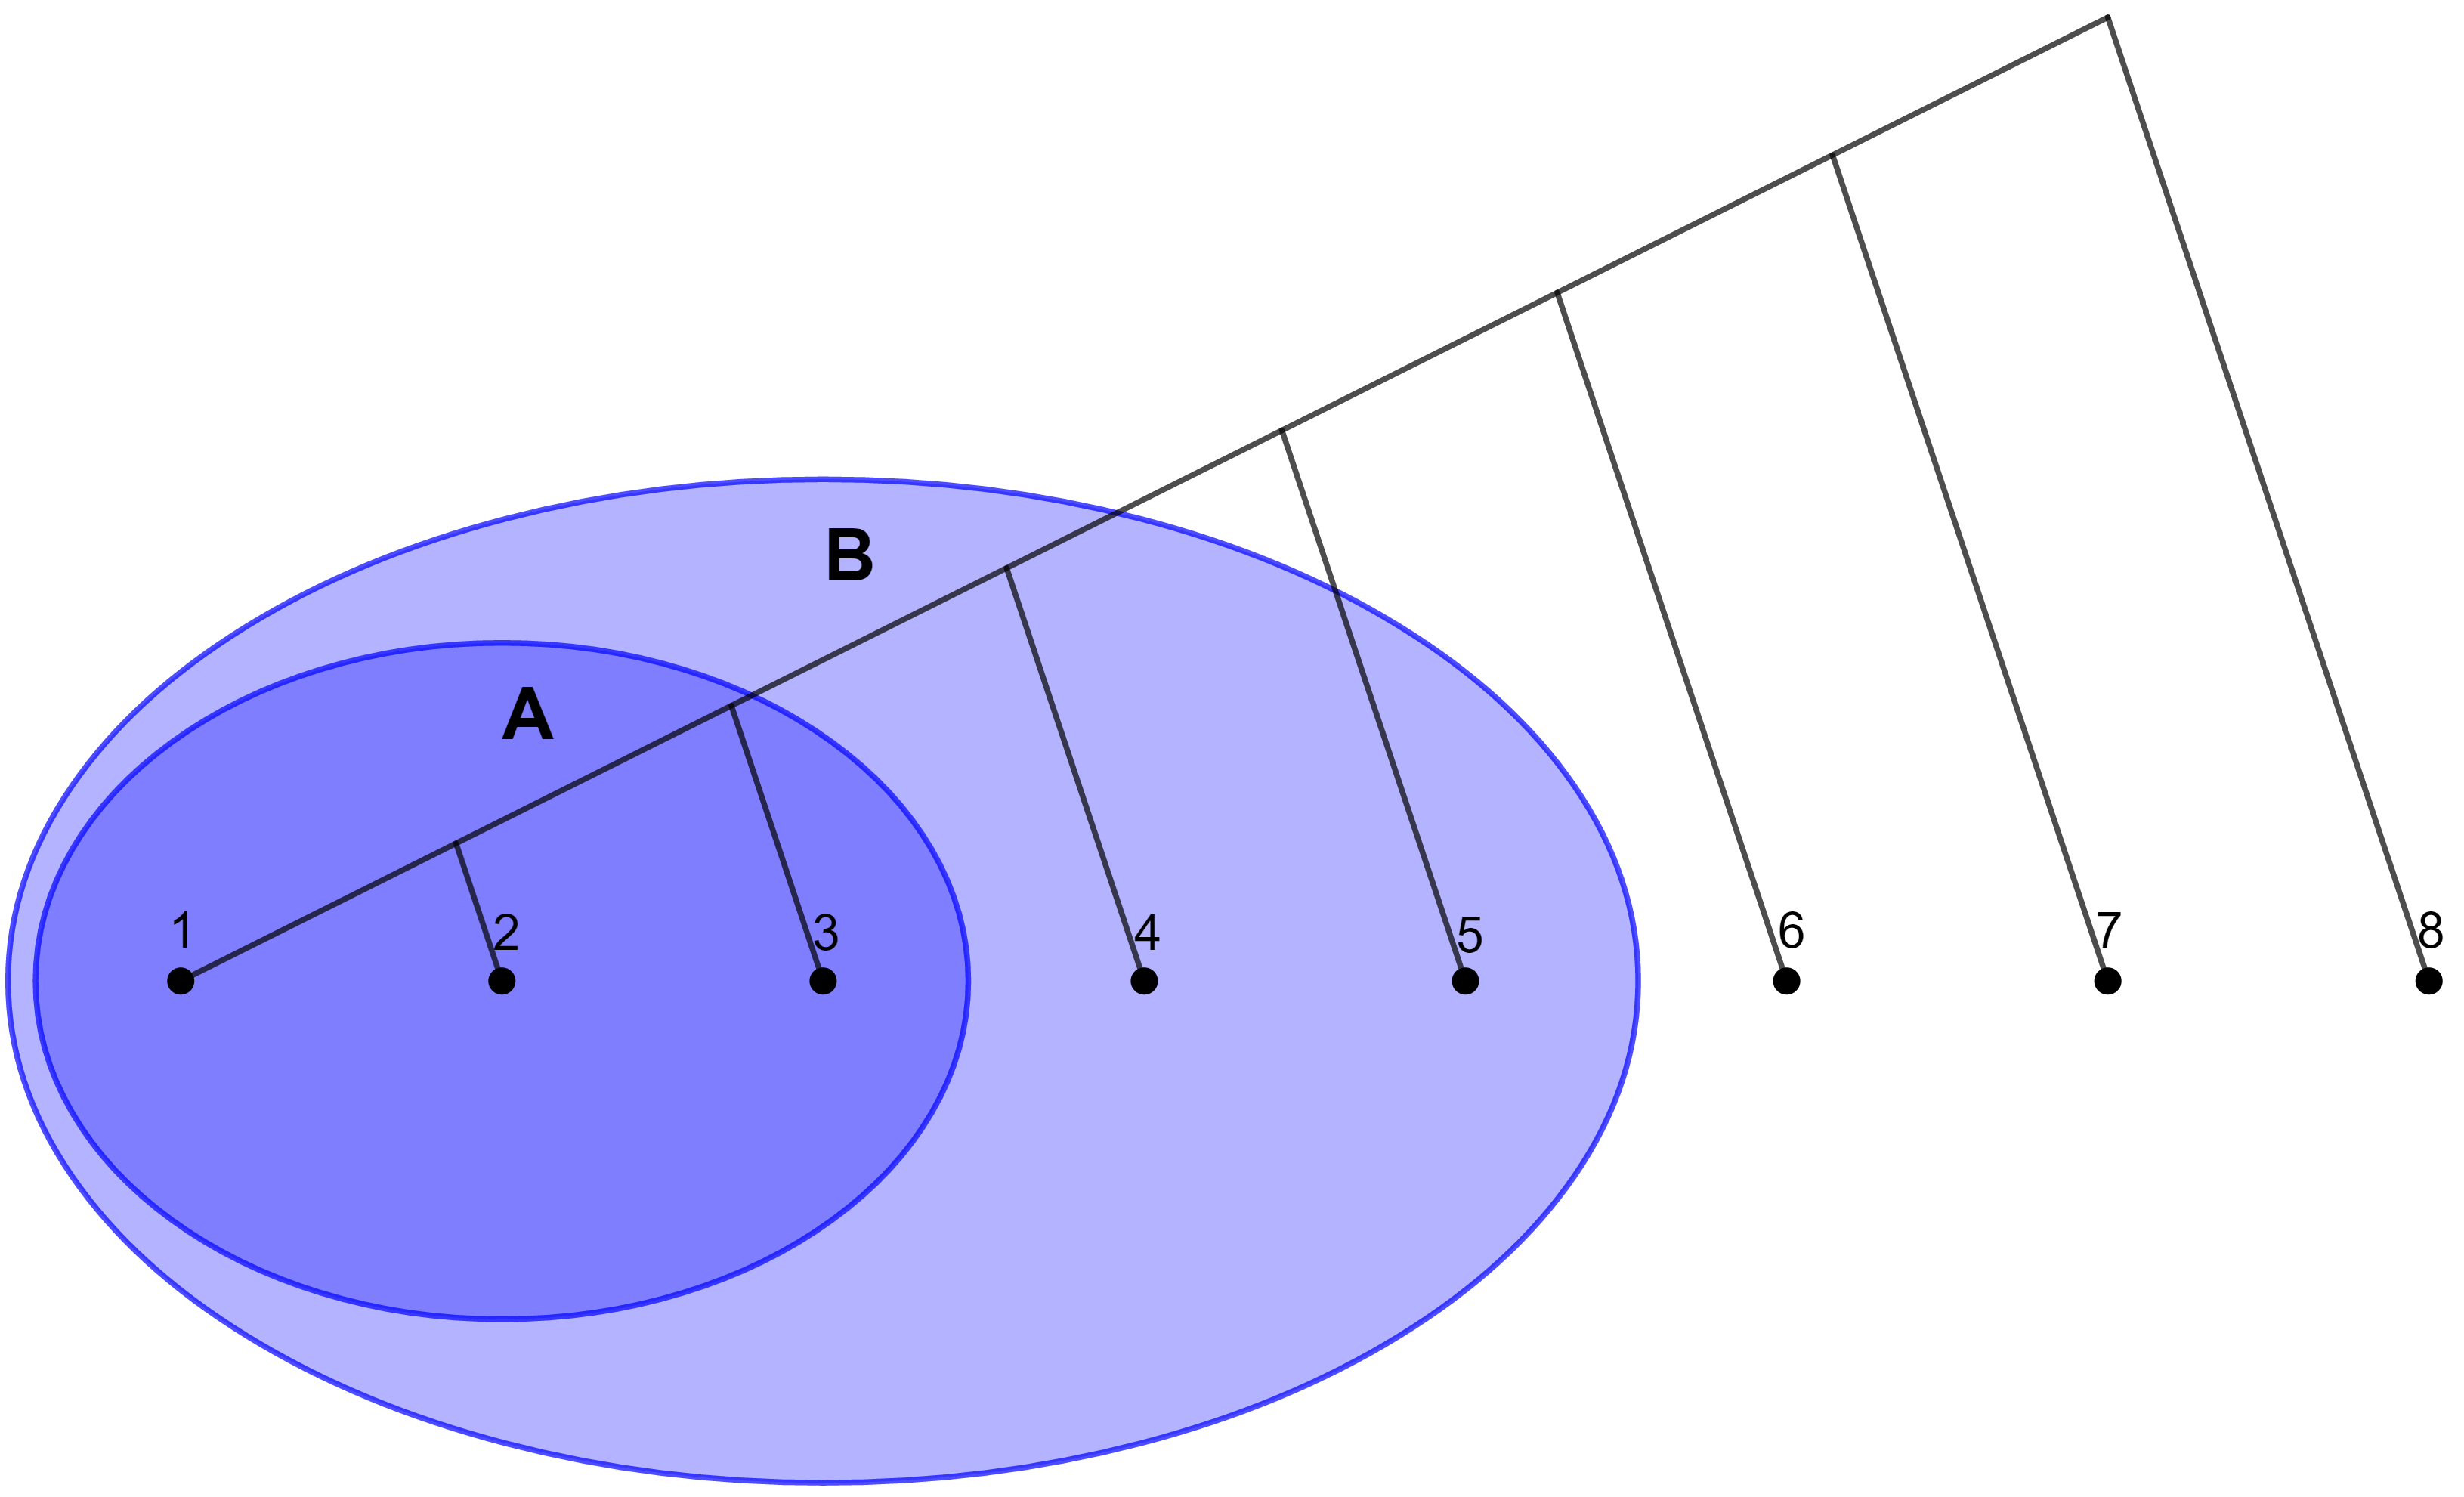
\includegraphics[width=.4\textwidth, margin=0pt 0pt 0pt 1ex,valign=m]{figures/python_tree_example_1.png}}
		& $\Bigg[ \, \bigg[ \, \underbrace{\Big[ \, \overbrace{\big[ \, [ \, [ 1 ], [ 2 ] \, ], [ 3 ] \, \big]}^{A}, [ 4 ] \, ], [ 5 ] \, \Big]}_{8}, [ 6 ] \, ], [ 7 ] \, \bigg], [ 8 ] \, \Bigg] $\\
		\cmidrule(r){1-1}\cmidrule(l){2-2} 
		{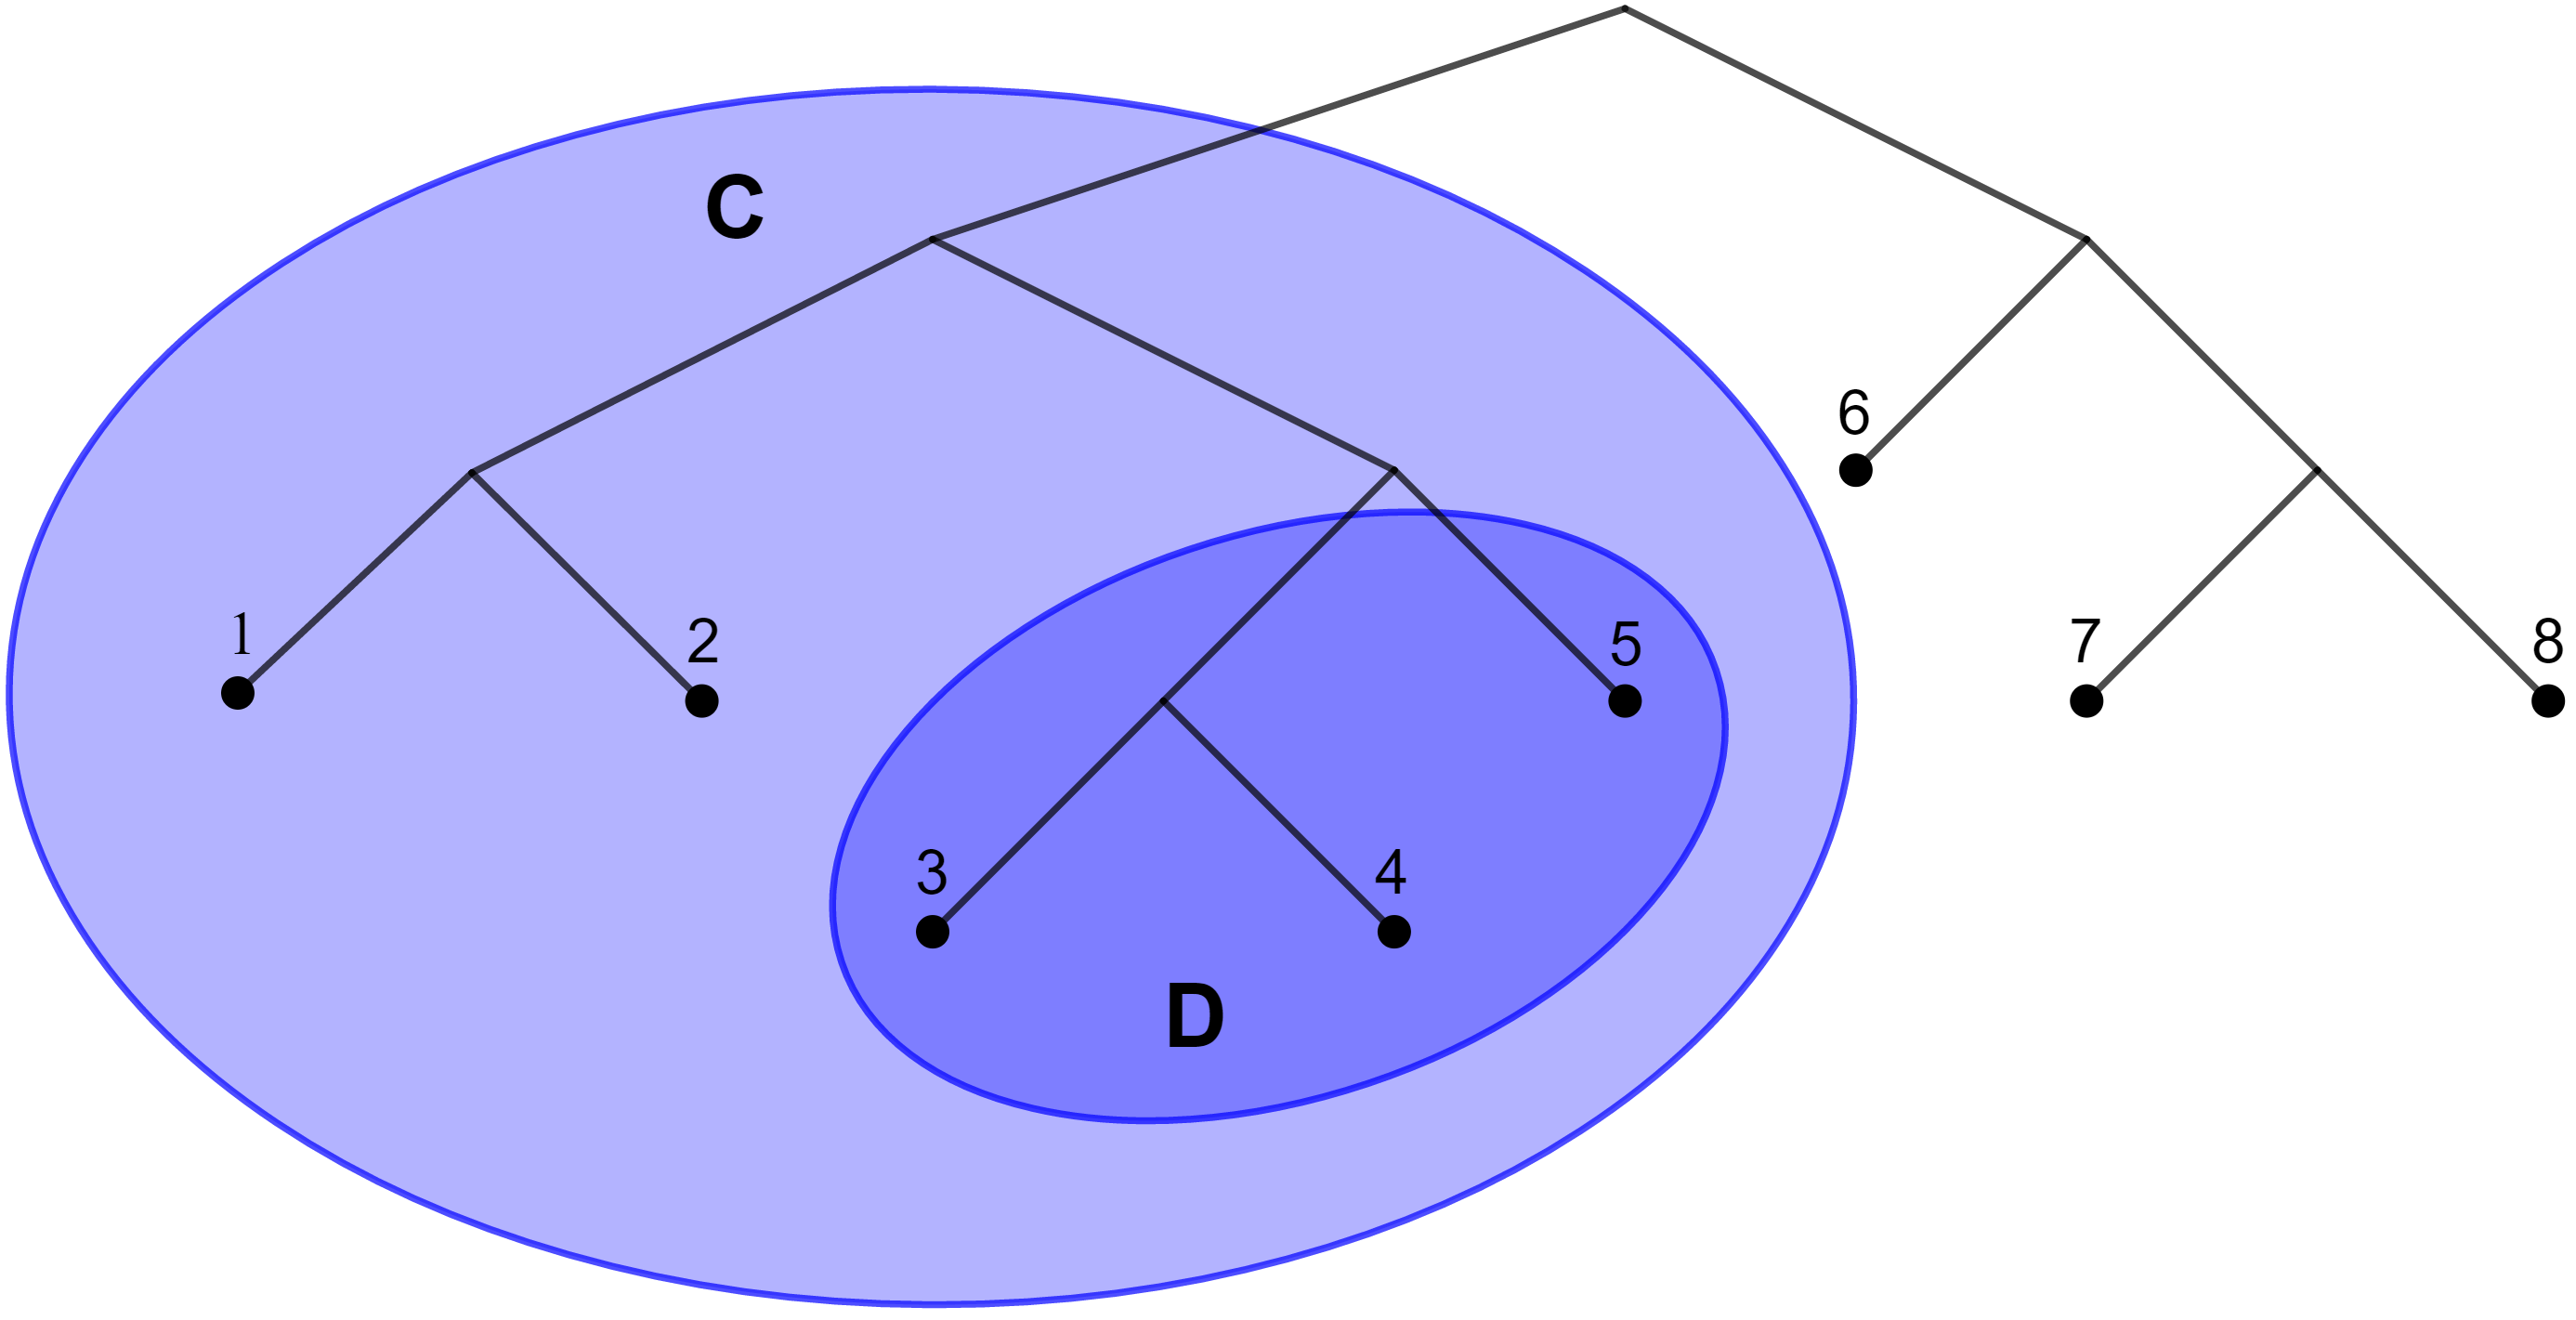
\includegraphics[width=.4\textwidth, margin=0pt 0pt 0pt 1ex,valign=m]{figures/python_tree_example_2.png}}
		& $\Bigg[ \, \underbrace{\bigg[ \, \Big[ \, [ 1 ], [ 2 ] \, \Big], \overbrace{\Big[ \, \big[ \, [ 3 ], [ 4 ] \, \big], [ 5 ] \, \Big]}^{D} \, \bigg]}_{C}, \bigg[ \, [ 6 ], \Big[ \, [ 7 ], [ 8 ] \, \Big]  \, \bigg] \, \Bigg]$\\
		\cmidrule(r){1-1}\cmidrule(l){2-2} 
		{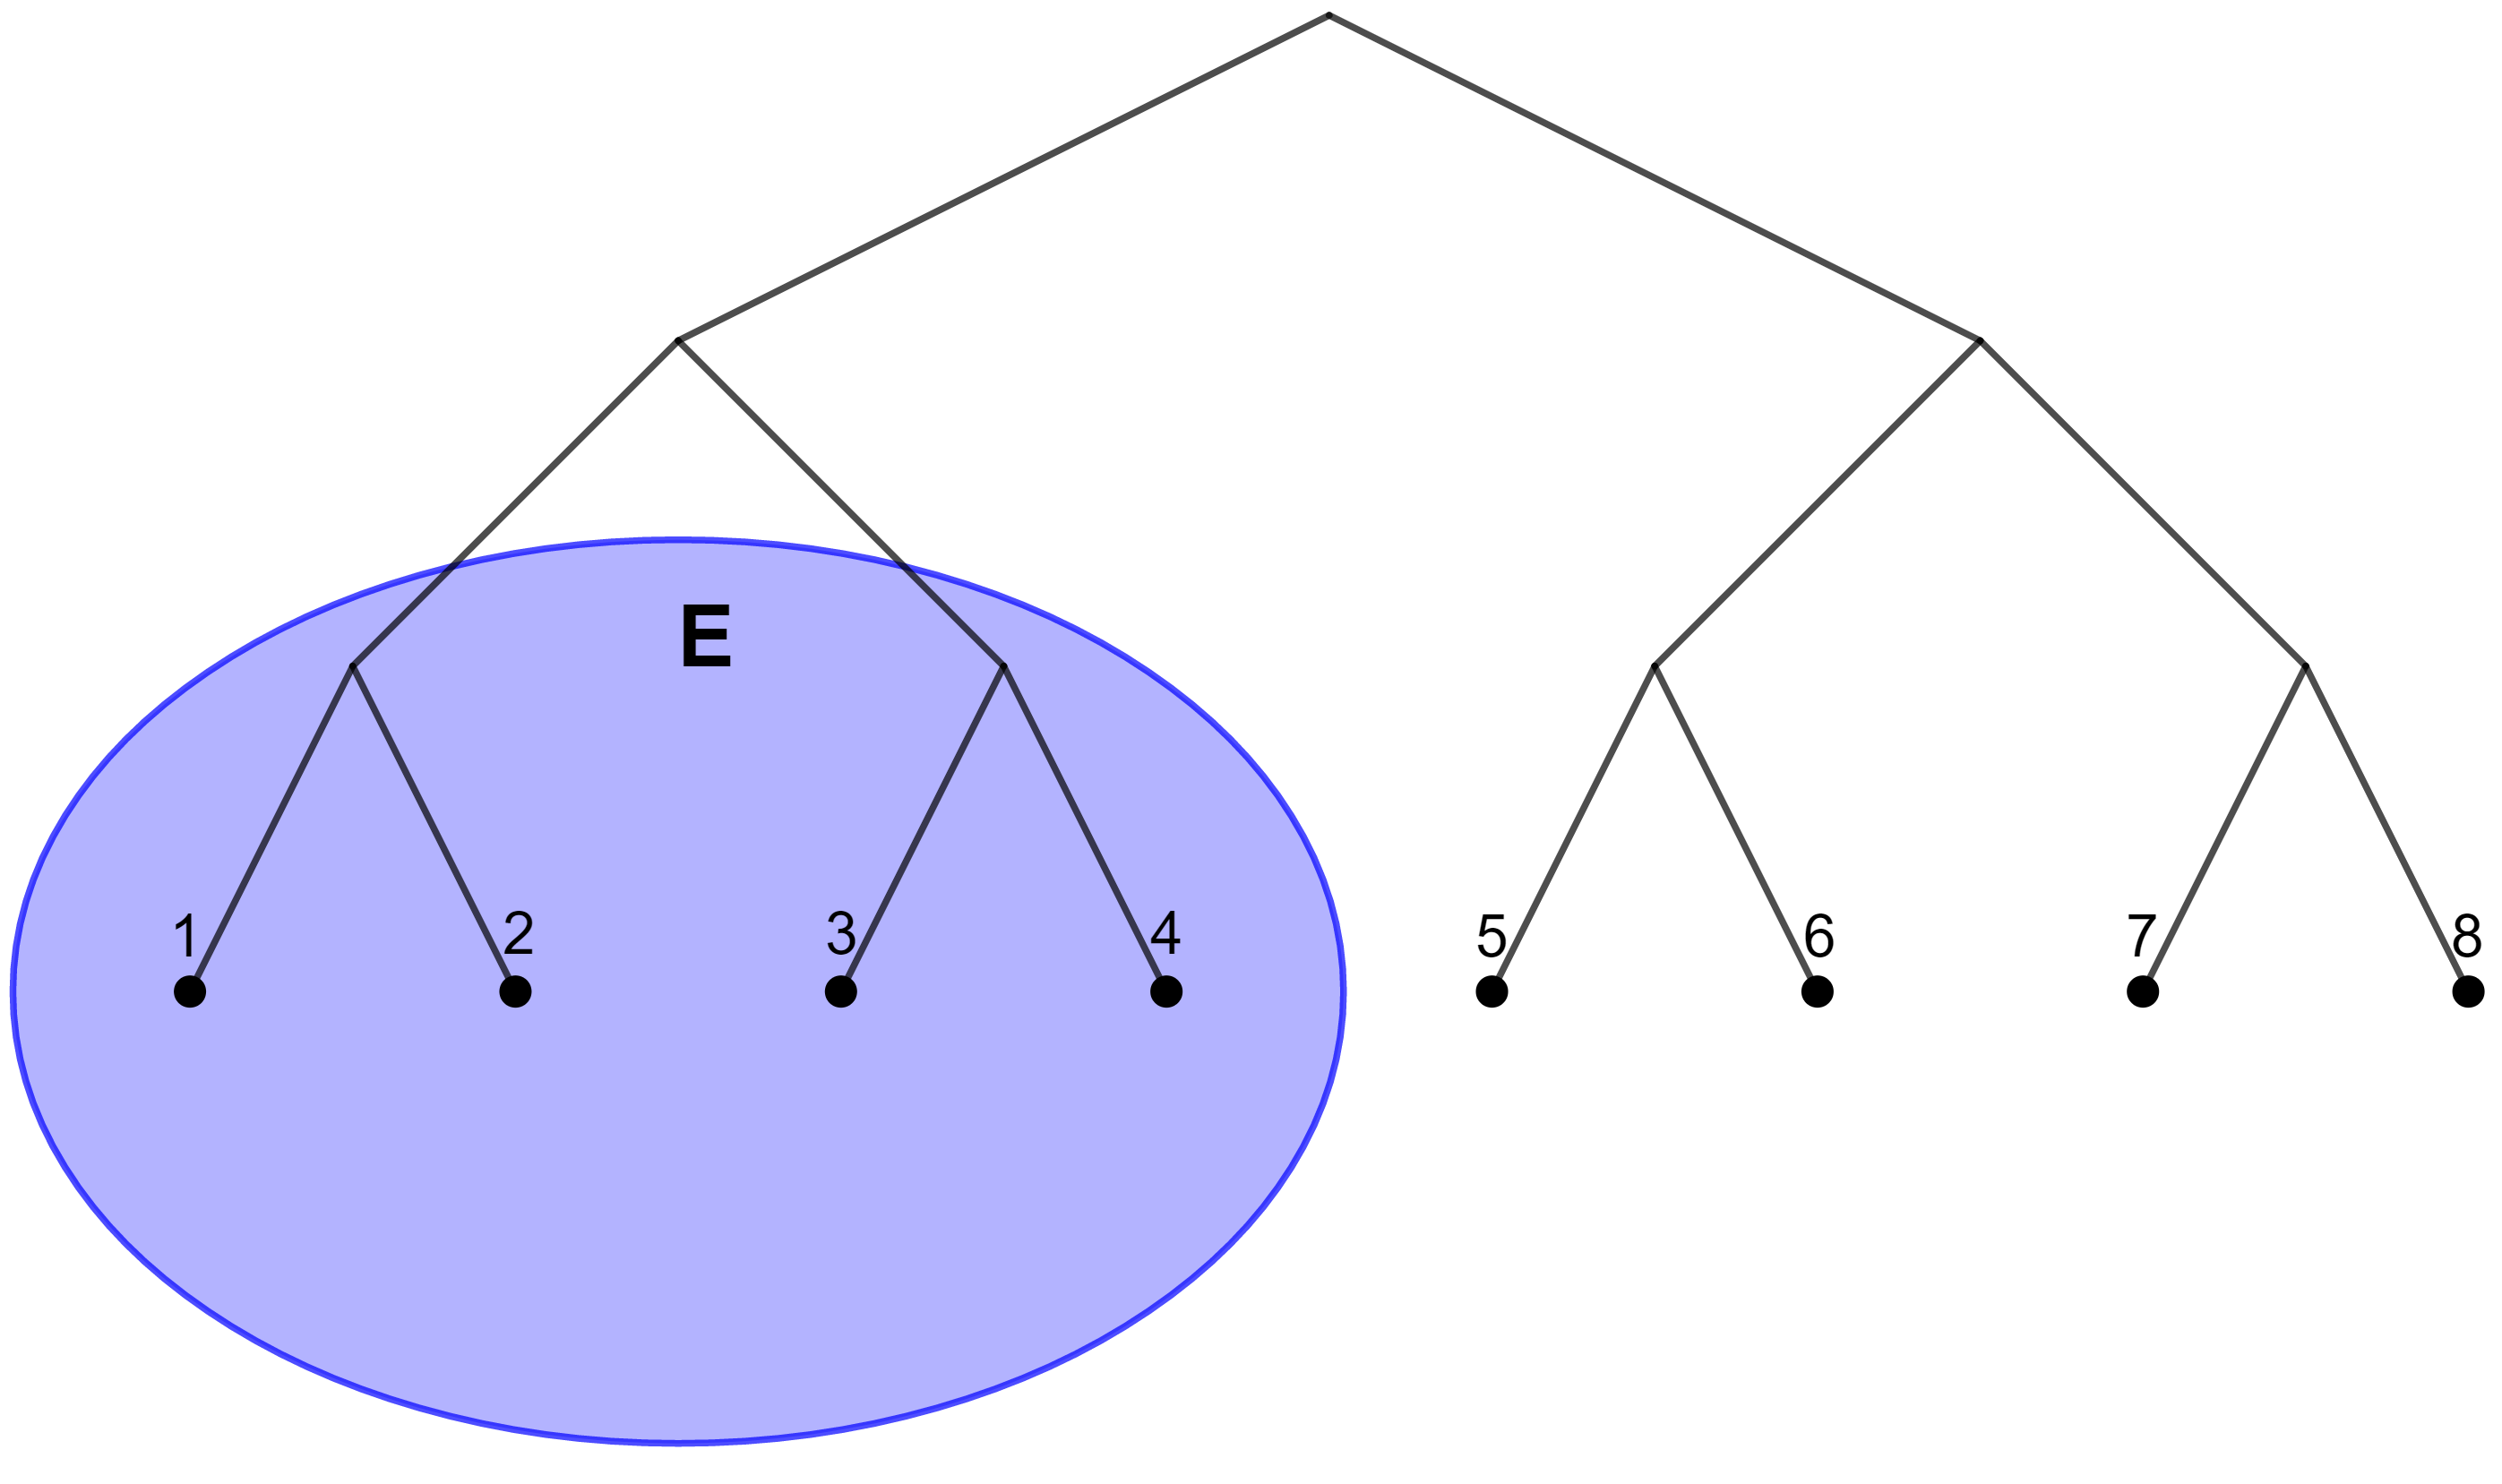
\includegraphics[width=.4\textwidth, margin=0pt 0pt 0pt 1ex,valign=m]{figures/python_tree_example_3.png}}
		& $\Bigg[ \, \underbrace{\bigg[ \, \Big[ \, [ 1 ], [ 2 ] \, \Big], \Big[ \, [ 3 ], [ 4 ] \, \Big] \, \bigg]}_{E}, \bigg[ \, \Big[ \, [ 5 ], [ 6 ] \, \Big], \Big[ \, [ 7 ], [ 8 ] \, \Big] \, \bigg] \, \Bigg]$\\
		
	\end{tabular}
\end{table}

\subsection{Distance Function}
The generalized Robinson-Foulds allows us to choose different distance measures. But since we have to compare our results with the tree edit distance, we need to choose a distance that counts wrong leaves. Therefore we stick with the introduced Robinson-Jaccard metric. We will compute the distances between trees with different values for the constant $k$. Thus we may see a pattern.

\section{Implementation Details}
We based our implementations of both the generalized Robinson-Foulds distance and the tree edit distance on the data structure used in an implementation of Shasha and Zhangs algorithm~\cite{Hen} introduced in Section~\ref{sec:saz}. For computing the generalized Robinson-Foulds distance we extended the data structure \textit{Node} of the above mentioned git repository to include the following functions:
\lstinputlisting[language=Python, caption=Scratch of the class ExtendedNode, label=lst:ExtNode]{figures/extended_node.py}
We based the computation of the generalized Robinson Foulds distance on the linear program introduced in Theorem~\ref{thm:gRF_LP}. We used a widely known, open-source library for linear programms within python, the PuLP- package. \\
Using this package enables us to create an instance of the LP-problem defined in~\ref{thm:gRF_LP} very easily. We start by definining the problem to be a binary LP and by initializing the decision variables $x_{i,j}$. For creating the restrictions we have to loop over all combinations of non-trivial clades in  $\mathcal{C}^*(T_1)$ and $\mathcal{C}^*(T_2)$ and calculate the value $\omega(C_i,C_j')$. Then we formulate the easy restriction from Inequalities~(\ref{eq:V_1}),(\ref{eq:V_2}). Last but not least we compute the set $\mathcal{I}$ to contain any possible combination of invalid edge combinations and add these combinations to the set of restrictions of the LP instance.

\section{Results}
As mentioned above we used the Jaccard metric to calculate the distance between sets of clusters. We used $k \in \{1,2,4,8,16,64\}$ and saw a pattern: Not only is the distance directly proportional to the value of $k$, but the overall distance tends to the standard Robinson Foulds distance very quickly as $k$ increases. \\
Furthermore, without regarding the quality of the results, we realized that the running time is a big problem for this approach. In Lemma~\ref{lem:numberOfRestrictions} we saw that the number of restrictions increases at a rate of (at least) $n^2\log^2(n)$. This leads to a huge ILP even for small trees with only $24$ leaves. Handling such instances with $24$ leaves on both trees already took my computer $500$ seconds. Increasing the number of leaves to $32$ on each tree leads to a running time of about $3100$ seconds. It already takes $22$ seconds to create the LP instance, however one has to be very patient to wait for a solution.\\
It is possible that more evolved linear programming packages solve these problems more efficiently. We tried to use Gurobi for comparison to the running time, but unfortunately this trial mainly delivered errors during the installation. It is possible, that a more advanced package like Gurobi would solve the LP instance faster, nevertheless, this approach doesn't seem to bring fast solutions for big problems as the number of restrictions increases extremely fast.